% Options for packages loaded elsewhere
\PassOptionsToPackage{unicode}{hyperref}
\PassOptionsToPackage{hyphens}{url}
%
\documentclass[
]{book}
\title{The Research Data Management Workbook}
\author{Kristin Briney}
\date{2023-08-18}

\usepackage{amsmath,amssymb}
\usepackage{lmodern}
\usepackage{iftex}
\ifPDFTeX
  \usepackage[T1]{fontenc}
  \usepackage[utf8]{inputenc}
  \usepackage{textcomp} % provide euro and other symbols
\else % if luatex or xetex
  \usepackage{unicode-math}
  \defaultfontfeatures{Scale=MatchLowercase}
  \defaultfontfeatures[\rmfamily]{Ligatures=TeX,Scale=1}
\fi
% Use upquote if available, for straight quotes in verbatim environments
\IfFileExists{upquote.sty}{\usepackage{upquote}}{}
\IfFileExists{microtype.sty}{% use microtype if available
  \usepackage[]{microtype}
  \UseMicrotypeSet[protrusion]{basicmath} % disable protrusion for tt fonts
}{}
\makeatletter
\@ifundefined{KOMAClassName}{% if non-KOMA class
  \IfFileExists{parskip.sty}{%
    \usepackage{parskip}
  }{% else
    \setlength{\parindent}{0pt}
    \setlength{\parskip}{6pt plus 2pt minus 1pt}}
}{% if KOMA class
  \KOMAoptions{parskip=half}}
\makeatother
\usepackage{xcolor}
\IfFileExists{xurl.sty}{\usepackage{xurl}}{} % add URL line breaks if available
\IfFileExists{bookmark.sty}{\usepackage{bookmark}}{\usepackage{hyperref}}
\hypersetup{
  pdftitle={The Research Data Management Workbook},
  pdfauthor={Kristin Briney},
  hidelinks,
  pdfcreator={LaTeX via pandoc}}
\urlstyle{same} % disable monospaced font for URLs
\usepackage{longtable,booktabs,array}
\usepackage{calc} % for calculating minipage widths
% Correct order of tables after \paragraph or \subparagraph
\usepackage{etoolbox}
\makeatletter
\patchcmd\longtable{\par}{\if@noskipsec\mbox{}\fi\par}{}{}
\makeatother
% Allow footnotes in longtable head/foot
\IfFileExists{footnotehyper.sty}{\usepackage{footnotehyper}}{\usepackage{footnote}}
\makesavenoteenv{longtable}
\usepackage{graphicx}
\makeatletter
\def\maxwidth{\ifdim\Gin@nat@width>\linewidth\linewidth\else\Gin@nat@width\fi}
\def\maxheight{\ifdim\Gin@nat@height>\textheight\textheight\else\Gin@nat@height\fi}
\makeatother
% Scale images if necessary, so that they will not overflow the page
% margins by default, and it is still possible to overwrite the defaults
% using explicit options in \includegraphics[width, height, ...]{}
\setkeys{Gin}{width=\maxwidth,height=\maxheight,keepaspectratio}
% Set default figure placement to htbp
\makeatletter
\def\fps@figure{htbp}
\makeatother
\setlength{\emergencystretch}{3em} % prevent overfull lines
\providecommand{\tightlist}{%
  \setlength{\itemsep}{0pt}\setlength{\parskip}{0pt}}
\setcounter{secnumdepth}{5}
\usepackage{booktabs}
\ifLuaTeX
  \usepackage{selnolig}  % disable illegal ligatures
\fi
\usepackage[]{natbib}
\bibliographystyle{plainnat}

\begin{document}
\maketitle

{
\setcounter{tocdepth}{1}
\tableofcontents
}
\hypertarget{about-this-book}{%
\chapter*{About this Book}\label{about-this-book}}
\addcontentsline{toc}{chapter}{About this Book}

\hypertarget{description}{%
\section*{Description}\label{description}}
\addcontentsline{toc}{section}{Description}

The Research Data Management Workbook is made up of a collection of exercises for researchers to improve their data management. The workbook contains exercises across the data lifecycle, though the range of activities is not comprehensive. Instead, exercises focus on discrete practices within data management that are structured and can be reproduced by any researcher.

The book is divided into chapters, roughly by phases of the data lifecycle, with one or more exercises in each chapter. Every exercise comes with a description of its value within data management, instructions on how to do the exercise, original source of the exercise (when applicable), and the exercise itself.

The workbook is intended as a supplement to existing data management education. If you would like to learn more about the principles of data management, please see the article ``Foundational Practices of Research Data Management'' \citep{briney_foundational_2020} or read the book ``Data Management for Researchers'' \citep{briney_data_2015}.

\hypertarget{edition}{%
\section*{Edition}\label{edition}}
\addcontentsline{toc}{section}{Edition}

The Research Data Management Workbook is currently in its beta edition, meaning I'm still tweaking the exercises and trying to catch stray typos. I'm more than happy to receive any feedback on the Workbook to improve it; you can message me at briney@caltech.edu.

\hypertarget{license}{%
\section*{License}\label{license}}
\addcontentsline{toc}{section}{License}

This book is available under a Creative Commons Attribution-NonCommercial (CC BY-NC) 4.0 International license.

I encourage you to use and adapt all of the exercises in this book for educational and personal use. Just remember to cite me:

\begin{itemize}
\tightlist
\item
  Briney, K. A. (2023). \emph{The Research Data Management Workbook.} Caltech Library.
\end{itemize}

\hypertarget{the-author}{%
\section*{The Author}\label{the-author}}
\addcontentsline{toc}{section}{The Author}

\begin{figure}
\centering
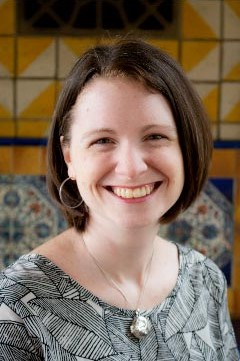
\includegraphics{images/00_KristinBriney.jpg}
\caption{Headshot of author, Kristin Briney}
\end{figure}

Kristin Briney is the Biology \& Biological Engineering Librarian at the California Institute of Technology and author of the books ``Data Management for Researchers'' \citep{briney_data_2015} and, with Becky Yoose, ``Managing Data for Patron Privacy'' \citep{briney_managing_2022}. She has a PhD in chemistry and an MLIS, both from the University of Wisconsin-Madison. Her research focuses on research data management, institutional data policy, and patron privacy vis-a-vis library data handling. Kristin is an advocate for the adoption of the international date standard ISO 8601 (YYYY-MM-DD) and likes to spend her free time making data visualizations out of yarn and fabric.

\hypertarget{introduction}{%
\chapter{Introduction}\label{introduction}}

\hypertarget{documentation}{%
\chapter{Documentation}\label{documentation}}

\hypertarget{lab-notebook}{%
\section{Evaluate a Laboratory Notebook}\label{lab-notebook}}

\textbf{\emph{Description:}} \emph{The laboratory or research notebook is a fundamental documentation method for many researchers. But for how ubiquitous the lab notebook is, documentation can sometimes be lacking. The ideal laboratory notebook allows someone with similar training as you to be able to follow everything you did in your research. This exercise prompts you to review an old entry within your laboratory notebook to evaluate if your documentation is sufficient for reproducing your work.}

\textbf{\emph{Instructions:}} \emph{You will need a laboratory notebook entry from 6-12 months ago to do this exercise. Once you have the entry, read through it to try to understand what you did on that day. Answer the exercise questions to evaluate the entry and identify any note keeping improvements to make.}

\begin{center}\rule{0.5\linewidth}{0.5pt}\end{center}

\textbf{Date of lab notebook entry being evaluated:} \_\_\_\_\_\_\_\_\_\_\_\_\_\_\_\_\_\_\_\_

\textbf{Read the entry and summarize the work you did on that date:}

~

~

~

\textbf{How easy was it to understand what you did from your notes? Could you reproduce your work solely from the information in your notes?}

~

~

~

\textbf{What worked well with your note keeping?}

~

~

~

\textbf{What would you improve about your note keeping?}

~

~

~

\textbf{List one change you plan to make to take better research notes:}

~

~

~

\hypertarget{readme-txt}{%
\section{Write a Project-Level README.txt}\label{readme-txt}}

\textbf{\emph{Description:}} \emph{Data files living on a computer often need extra documentation for someone to understand what research they correspond to. In particular, it is useful to record the most basic project information and store it in the top-level folder of each research project. This can be done with a README.txt. The name, ``README'', indicates that the file conveys important information and the file type, TXT, can be opened by many different software programs, making the content maximally accessible. This exercise walks you through the key information needed in a project-level README.txt file. The same information can also be recorded at the front of a physical laboratory notebook.}

\textbf{\emph{Instructions:}} \emph{Pick a research project and answer the following questions. Copy all of the text into a TXT file and save it with the name ``README.txt''. Store this file in the top-level of the project folder on your computer, alongside the project files.}

\textbf{\emph{Source:}} \emph{This exercise was adapted from the ``Project Close Out Checklist'' \citep{briney_project_2020}.}

\begin{center}\rule{0.5\linewidth}{0.5pt}\end{center}

\textbf{What is the title of the project?}

~

~

~

\textbf{What is the project description?}

~

~

~

\textbf{What is the time period the project was done over?}

~

~

~

\textbf{Who worked on the project?}

~

~

~

\textbf{Where are the files are stored?}

~

~

~

\textbf{How are files organized? Are any naming conventions used and, if so, what are they (see \protect\hyperlink{file-organization-and-naming}{Chapter 3})?}

~

~

~

\hypertarget{data-dictionary}{%
\section{Create a Data Dictionary}\label{data-dictionary}}

\textbf{\emph{Description:}} \emph{Ideally, a spreadsheet is formatted with a row of variable names at the top, followed by rows of data going down. This makes easy for data to be used in any data analysis software (interoperability is a good thing) but makes it impossible to document a spreadsheet within the file itself. For this reason, it's useful to create a data dictionary to describe the spreadsheet so that others can interpret the data. This exercise walks you through the major information you should record for each variable in the spreadsheet, adding up to a complete dictionary to accompany the spreadsheet file.}

\textbf{\emph{Instructions:}} \emph{Fill out the information in each row for each variable in the spreadsheet; note that you will likely have more variables than columns in this table. Copy this information into a text document and save it next to the spreadsheet. It is useful to save the data dictionary with the same root name as its data file by appending ``\_dictionary'' on the end of the file name; for example, the data dictionary for the file ``myData.xlsx'' would be ``myData\_dictionary.txt''.}

\textbf{\emph{Source:}} \emph{This exercise was adapted from ``Leveling Up Data Management'' \citep{briney_leveling_2023}.}

\begin{center}\rule{0.5\linewidth}{0.5pt}\end{center}

\begin{tabular}{l|l|l|l}
\hline
Question & Variable1 & Variable2 & Variable3\\
\hline
Variable name &  &  & \\
\hline
Variable description &  &  & \\
\hline
Variable units &  &  & \\
\hline
Relationship to other variables &  &  & \\
\hline
Variable coding values and meanings &  &  & \\
\hline
Known issues with the data &  &  & \\
\hline
Anything else to know about the data? &  &  & \\
\hline
\end{tabular}

\hypertarget{file-organization-and-naming}{%
\chapter{File Organization and Naming}\label{file-organization-and-naming}}

\hypertarget{file-organization}{%
\section{Set Up a File Organization System}\label{file-organization}}

\textbf{\emph{Description:}} \emph{Implementing a file organization system is the first step toward creating order for your research data. Well-organized files make it easier to find the data you need without spending lots of time searching your computer. Every researcher organizes their files slightly differently, but the actual organizational system is less important that having a place where all of your files should logically go. This exercise prompts you to brainstorm organizational groupings and hierarchies to come up with an order for managing your research data.}

\textbf{\emph{Instructions:}} \emph{This is a card-sorting exercise, meaning you will need a stack of note cards or post-it notes to do this activity, ideally in three different colors. Follow the instructions to label cards and move them around until you develop your organizational system. There is no one correct way to do this so feel free to play around, add new cards, and move cards however you want! Once you put your new organizational system into place, be sure to always put your files where they're supposed to go.}

\begin{center}\rule{0.5\linewidth}{0.5pt}\end{center}

\begin{enumerate}
\def\labelenumi{\arabic{enumi}.}
\tightlist
\item
  Take a stack of note cards or post-it notes in the first color and write the following labels on one card each, omitting any file types that you do not use in your research:

  \begin{itemize}
  \tightlist
  \item
    Raw data
  \item
    Analyzed data
  \item
    Code
  \item
    Protocols
  \item
    Article drafts
  \item
    Figures
  \item
    Your publications
  \item
    Literature PDFs
  \item
    Grant documents
  \item
    Research notes
  \end{itemize}
\item
  Move cards around and group together file-type cards that you want to store together. Files that will be stored near each other in a folder hierarchy, but not together, should be placed near each other while file types expected to be stored completely separately should be away from other cards.
\item
  Create hierarchies in file organization by adding new ``folder'' cards in one of two types; use different colored cards for each folder type:

  \begin{itemize}
  \tightlist
  \item
    Cards in the second color represent a single folder. These should be labeled with the folder name in quotations (e.g.~``Literature'' or ``My publications'').
  \item
    Cards in the third color represent a group of folders, such as for folders organized by date or by project. Use only one card to represent the organizational pattern that will be repeated. These cards should be labeled with the organizational system in square brackets (e.g.~{[}By date{]} or {[}By project{]}).
  \end{itemize}
\item
  Move existing file-type cards/groups of file-type cards underneath the new folder cards to show that a file type will be saved in a specific folder or group of folders. Organizational-group folders (cards in the third color) only need to be represented once in the card sorting, as they are assumed to represent multiple folders on a computer.
\item
  Make copies of any type of card and add folder levels, as needed. Adjust placement and hierarchies until you are happy with the organizational system you developed.
\item
  Record your organizational system in your lab notebook or in a \protect\hyperlink{readme-txt}{README.txt}.
\end{enumerate}

\hypertarget{file-naming}{%
\section{Create a File Naming Convention}\label{file-naming}}

\textbf{\emph{Description:}} \emph{File naming conventions are a simple way to add order to your files and help to find them later. Rich and descriptive file names make it easier to search for files, understand at a glance what they contain, and tell related files apart.}

\begin{figure}
\centering
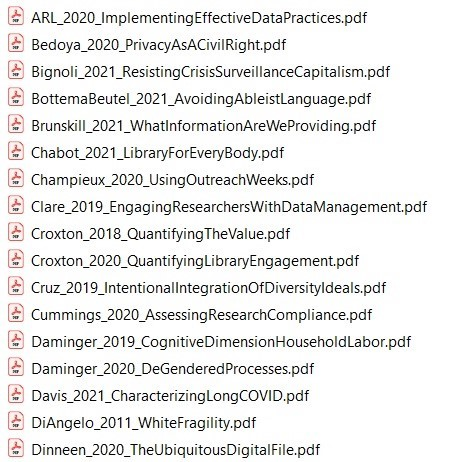
\includegraphics{images/03_FileNaming.jpg}
\caption{Screenshot of pdf's with consistent file names using the convention FirstAuthorLastName\_YEAR\_ShortTitle.pdf}
\end{figure}

\textbf{\emph{Instructions:}} \emph{This exercise guides researchers through the process of creating a file naming convention for a group of related files. Fill in each section for a group of related files following the instructions; an example for microscopy files is provided. This exercise may be redone as needed, as different groups of files require different naming conventions.}

\textbf{\emph{Source:}} \emph{This exercise is based on the ``File Naming Convention Worksheet'' \citep{briney_file_2020}.}

\begin{center}\rule{0.5\linewidth}{0.5pt}\end{center}

\textbf{1. What group of files will this naming convention cover?}

You can use different conventions for different file sets.

\emph{Example: This convention will apply to all of my microscopy files, from raw image through processed image.}

~

~

~

\textbf{2. What information (metadata) is important about these files and makes each file distinct?}

Ideally, pick three pieces of metadata; use no more than five. This metadata should be enough for you to visually scan the file names and easily understand what's in each one.

\emph{Example: For my images, I want to know date, sample ID, and image number for that sample on that date.}

\begin{enumerate}
\def\labelenumi{\arabic{enumi}.}
\tightlist
\item
\item
\item
\item
\item
\end{enumerate}

\textbf{3. Do you need to abbreviate any of the metadata or encode it?}

If any of the metadata from step 2 is described by lots of text, decide what shortened information to keep. If any of the metadata from step 2 has regular categories, standardize the categories and/or replace them with 2- or 3-letter codes; be sure to document these codes.

\emph{Example: Sample ID will use a code made up of: a 2-letter project abbreviation (project 1 = P1, project 2 = P2); a 3-letter species abbreviation (mouse = ``MUS'', fruit fly = ``DRS''); and 3-digit sample ID (assigned in my notebook).}

~

~

~

\textbf{4. What is the order for the metadata in the file name?}

Think about how you want to sort and search for your files to decide what metadata should appear at the beginning of the file name. If date is important, use ISO 8601-formatted dates (YYYYMMDD or YYYY-MM-DD) at the beginning of the file names so dates sort chronologically.

\emph{Example: My sample ID is most important so I will list it first, followed by date, then image number.}

\begin{enumerate}
\def\labelenumi{\arabic{enumi}.}
\tightlist
\item
\item
\item
\item
\item
\end{enumerate}

\textbf{5. What characters will you use to separate each piece of metadata in the file name?}

Many computer systems cannot handle spaces in file names. To make file names both computer- and human-readable, use dashes (-), underscores (\_), and/or capitalize the first letter of each word in the file names.

\emph{Example: I will use underscores to separate metadata and dashes between parts of my sample ID.}

~

~

~

\textbf{6. Will you need to track different versions of each file?}

You can track versions of a file by appending version information to end of the file name. Consider using a version number (e.g.~``v01'') or the version date (use ISO 8601 format: YYYYMMDD or YYYY-MM-DD).

\emph{Example: As each image goes through my analysis workflow, I will append the version type to the end of the file name (e.g.~``\_raw'', ``\_processed'', and ``\_composite'').}

~

~

~

\textbf{7. Write down your naming convention pattern.}

Make sure the convention only uses alphanumeric characters, dashes, and underscores. Ideally, file names will be 32 characters or less.

\emph{Example: My file naming convention is ``SA-MPL-EID\_YYYYMMDD\_\#\#\#\_status.tif'' Examples are ``P1-MUS-023\_20200229\_051\_raw.tif'' and ``P2-DRS-285\_20191031\_062\_composite.tif''.}

~

~

~

\textbf{8. Document this convention in a README.txt (or save this worksheet) and keep it with your files.}

~

~

~

\hypertarget{data-storage}{%
\chapter{Data Storage}\label{data-storage}}

\hypertarget{storage}{%
\section{Store and Back Up the Data}\label{storage}}

\textbf{\emph{Description:}} \emph{Research data needs to be stored and backed up reliably so that important data is not lost. But storage is commonly a challenge, as institutions don't always offer uniform options for storage and backup. This exercise prompts you to examine the storage and backup systems available to you, either free or paid, as well as options outside of your institution, before determining which is the best set of options for your data.}

\textbf{\emph{Instructions:}} \emph{Fill out the first three tables for storage and backup systems that are: 1) institutional and free; 2) institutional and paid; and 3) outside of your institution. Examine all of the options, evaluating them based on the criteria listed below the first three tables to pick your ideal storage and backup configuration. \textbf{Note that this exercise works best for data under 1 TB in size that has no security restrictions.}}

\begin{center}\rule{0.5\linewidth}{0.5pt}\end{center}

\textbf{What storage or backup systems are already available to you, such as through your institution or workplace, at no cost?}

\begin{tabular}{l|l|l|l}
\hline
Question & System1 & System2 & System3\\
\hline
System name &  &  & \\
\hline
Is it storage or backup? &  &  & \\
\hline
What is the hardware type? &  &  & \\
\hline
Is the system backed up? &  &  & \\
\hline
For backup systems, is backup automatic? &  &  & \\
\hline
Is the system local or remote? &  &  & \\
\hline
How is there a limit to storage capacity? &  &  & \\
\hline
Who manages the system? &  &  & \\
\hline
Is it easy or difficult to use? &  &  & \\
\hline
\end{tabular}

\textbf{What storage or backup systems are available to you, such as through your institution or workplace, at a cost?}

\begin{tabular}{l|l|l|l}
\hline
Question & System1 & System2 & System3\\
\hline
System name &  &  & \\
\hline
Is it storage or backup? &  &  & \\
\hline
What is the cost? &  &  & \\
\hline
What is the hardware type? &  &  & \\
\hline
Is the system backed up? &  &  & \\
\hline
For backup systems, is backup automatic? &  &  & \\
\hline
Is the system local or remote? &  &  & \\
\hline
How is there a limit to storage capacity? &  &  & \\
\hline
Who manages the system? &  &  & \\
\hline
Is it easy or difficult to use? &  &  & \\
\hline
\end{tabular}

\textbf{Are there other storage or backup systems that you can use? }

\begin{tabular}{l|l|l|l}
\hline
Question & System1 & System2 & System3\\
\hline
System name &  &  & \\
\hline
Is it storage or backup? &  &  & \\
\hline
What is the cost? &  &  & \\
\hline
What is the hardware type? &  &  & \\
\hline
Is the system backed up? &  &  & \\
\hline
For backup systems, is backup automatic? &  &  & \\
\hline
Is the system local or remote? &  &  & \\
\hline
How is there a limit to storage capacity? &  &  & \\
\hline
Who manages the system? &  &  & \\
\hline
Is it easy or difficult to use? &  &  & \\
\hline
\end{tabular}

\textbf{Optimize your storage and backups on the following considerations:}

\begin{enumerate}
\def\labelenumi{\arabic{enumi}.}
\tightlist
\item
  You need one storage system that will hold all of your data files, is easy to use, and is managed by someone you trust.
\item
  You need at least one backup -- preferably two -- that will hold all of your data files, is managed by someone you trust, is easy to use, and backs up automatically.
\item
  At least one backup should be in a different location than your main storage system for disaster resiliency.
\item
  Balance cost with making sure that storage/backup systems are managed by trustworthy parties and are not difficult to use.
\end{enumerate}

\textbf{Pick your storage and backup systems:}

\begin{tabular}{l|l|l}
\hline
Storage & Backup1 & Backup2\\
\hline
\&nbsp; & \&nbsp; & \&nbsp;\\
\hline
\end{tabular}

\hypertarget{backup}{%
\section{Test Your Backup}\label{backup}}

\textbf{\emph{Description:}} \emph{Backups are super important for your data, so it's always good to test that your backups are still working. Nothing is worse than losing your data from your primary storage and then realizing that your backup isn't working either. Beyond checking that your backup is working, it's also good to know how to recover your files so that you don't have to learn this for the first time while panicking about lost data. This short exercise walks you through getting a file off your backup to test that it is working and to learn how the data-recovery process works.}

\textbf{\emph{Instructions:}} \emph{Pick a backup system and a file to recover and work through the steps. The hard part of this exercise is finding instructions for file recovery and recovering the file, which vary by backup system.}

\begin{center}\rule{0.5\linewidth}{0.5pt}\end{center}

\begin{enumerate}
\def\labelenumi{\arabic{enumi}.}
\tightlist
\item
  Identify where your data is backed up.
\item
  Find instructions for recovering data from your backup system.
\item
  Pick a data file from your computer.
\item
  Follow the instructions from step 2 to get a copy of the data file from step 3 out of your backup system.
\item
  If this process didn't work, fix your backup system. If this process did work, congrats your backup is working and you know how to recover your files!
\end{enumerate}

\hypertarget{data-management}{%
\chapter{Data Management}\label{data-management}}

\hypertarget{living-dmp}{%
\section{Write a Living Data Management Plan (DMP)}\label{living-dmp}}

\textbf{\emph{Description:}} \emph{Many researchers are aware of the two-page data management plan (DMP) for a grant application, but you may not be aware of the more useful type of DMP: a living DMP. This document describes how data will be actively managed during a project and may be updated whenever necessary to reflect current data practices. A living DMP is a useful touchstone for understanding where data lives, how it's labelled, how it moves through the research process, and who will oversee the data management. This exercise guides you through the process of creating a living DMP for your research.}

\textbf{\emph{Instructions:}} \emph{Pick a project and answer the following questions to build your living DMP. This DMP may be changed at any time to improve practices. If you are doing collaborative research, work through this exercise with your collaborators to agree on shared conventions.}

\begin{center}\rule{0.5\linewidth}{0.5pt}\end{center}

\textbf{Write a short summary of what project this DMP is for:}

~

~

~

\textbf{How will your data be organized? (See \protect\hyperlink{file-organization}{Exercise 3.1: Set Up a File Organization System}.)}

~

~

~

\textbf{What naming convention(s) will you use for your data? (See \protect\hyperlink{file-naming}{Exercise 3.2: Create a File Naming Convention}.)}

~

~

~

\textbf{Where will data be stored? How will data be backed up? (See \protect\hyperlink{storage}{Exercise 4.1: Store and Back Up the Data}.)}

~

~

~

\textbf{How will you document your research? Where will your research notes be stored?}

~

~

~

\textbf{How will data move through the collection and analysis pipelines?}

~

~

~

\textbf{Do you need to do any version control on your files? How will that be done?}

~

~

~

\textbf{As necessary, record any project roles and responsibilities around data management:}

~

~

~

\hypertarget{data-governance}{%
\section{Determine Data Stewardship}\label{data-governance}}

\textbf{\emph{Description:}} \emph{It is often helpful to be up front about requirements and permissions around research data. This exercise encourages you to discuss these issues with supervisors and peers to make sure that there are no misunderstandings about who has what rights to use, retain, and share data.}

\textbf{\emph{Instructions:}} \emph{Determine which research data should be discussed. Bring together the Principle Investigator, the researcher collecting the data, and anyone else who works with that data. As a group, answer the questions in the exercise, making sure that everyone agrees on the final decisions. Record the results of the discussion and save them with the project files.}

\textbf{\emph{Source:}} \emph{This exercise was adapted from the ``Project Close Out Checklist'' \citep{briney_project_2020}.}

\begin{center}\rule{0.5\linewidth}{0.5pt}\end{center}

\textbf{What data is being discussed?}

~

~

~

\textbf{Are there security or intellectual property restrictions on the data and, if so, what are they?}

~

~

~

\textbf{Are there any requirements to publicly share the data and, if so, what are they?}

~

~

~

\textbf{Who will store the copy of record of the data and for how long?}

~

~

~

\textbf{Who is allowed to keep a copy of the data after the project ends? Which data?}

~

~

~

\textbf{Who is allowed to reuse the data after the project ends? Are there any requirements for reuse, such as co-authorship?}

~

~

~

\textbf{Who keeps any physical research notebooks after the project ends?}

~

~

~

\hypertarget{data-sharing}{%
\chapter{Data Sharing}\label{data-sharing}}

\hypertarget{data-repository}{%
\section{Pick a Data Repository}\label{data-repository}}

\textbf{\emph{Description:}} \emph{It can be difficult to know where to share research data as so many sharing platforms are available. Current guidance is to deposit data in data repository that will give you a DOI. This exercise guides you through the process of picking a data repository, starting with repositories for very specific types of data and defaulting to generalist data repositories. Note that some repositories charge fees for deposit, most often for large data (500 GB or larger).}

\textbf{\emph{Instructions:}} \emph{Identify the data that needs to be shared and work through repository selection from discipline-specific data repositories to more general data repositories. Once you have identified a repository for all of your data, the exercise is over and you do not need to answer any further questions. Note that, depending on data types, you may need to deposit your data into multiple repositories (for example, a discipline-specific repository for one type of data and an institutional data repository for the rest of the data).}

\begin{center}\rule{0.5\linewidth}{0.5pt}\end{center}

\textbf{Identify all of the data that needs to be shared.}

~

~

~

\textbf{Is there a known disciplinary data repository for some or all of the data? For example, is there a data repository used by everyone in your research area or required for your data type by your funder?}

If so, deposit some or all of your data there. End the exercise if the repository will accept all of your data or keep going if there is still some data left to deposit.

~

~

~

\textbf{Review the \href{https://journals.plos.org/plosone/s/recommended-repositories}{list of recommended data repositories from PLOS}. Is there a logical disciplinary data repository for some or all of your data?}

If so, deposit some or all of your data there. End the exercise if you have shared all of your data or keep going if there is still some data left to deposit.

~

~

~

\textbf{Does your institution have a data repository?}

If so, deposit your data there and end the exercise.

~

~

~

\textbf{Do you have a preferred \href{https://sharing.nih.gov/data-management-and-sharing-policy/sharing-scientific-data/generalist-repositories}{generalist data repository}?}

If so, deposit your data there and end the exercise.

~

~

~

\textbf{Pick a \href{https://sharing.nih.gov/data-management-and-sharing-policy/sharing-scientific-data/generalist-repositories}{generalist data repository} and deposit your data.}

~

~

~

\hypertarget{share-data}{%
\section{Share Data}\label{share-data}}

\textbf{\emph{Description:}} \emph{Data sharing is becoming common and expected by funding agencies and journals. While the process of depositing data into a data repository will vary between repositories, there are some common actions that should be taken to prepare data for sharing. This exercise walks you through these standard requirements for sharing data.}

\textbf{\emph{Instructions:}} \emph{This checklist enumerates the necessary steps and decisions to deposit data supporting a research article into a data repository. Identify the data to be shared and work through the list. Note that, if data will be shared as multiple deposits or in multiple repositories, the checklist should be worked separately for each group of data.}

\begin{center}\rule{0.5\linewidth}{0.5pt}\end{center}

\textbf{Data Selection}

□ Select data that reproduces published results.

□ Perform quality control on the data files.

□ Convert data in proprietary file types to open file types, as appropriate; see \protect\hyperlink{file-type}{Exercise 7.2: Convert Data File Types}.

□ Determine if data will be shared in one group or as several deposits. If there will be multiple deposits in one repository or data will be divided across more than one data repository, work through the remainder of the checklist separately for each group of shared files.

\textbf{Data Documentation}

□ Document any spreadsheet data with a data dictionary (see \protect\hyperlink{data-dictionary}{Exercise 2.3: Create a Data Dictionary}). The data dictionary should be shared with the other files.

□ Write a brief description of each data file, including any data dictionaries, and what it contains. Save this information in a README.txt file and share it with the other files.

□ Write a brief description of the overall data to be used during deposit process for the dataset Description/Abstract.

\textbf{Sharing Information (Metadata)}

□ Give the dataset a title. Default is ``Data from: {[}name of the article{]}''.

□ Determine who will be listed as authors of the data and in what order; this may be different than the authors of the article.

□ Chose a license for reuse. Default is CC0 \citep{creative_commons_wiki_cc0_2014}.

\textbf{Deposit Data}

□ Pick a data repository using \protect\hyperlink{data-repository}{Exercise 6.1: Pick a Data Repository}

□ Deposit the data and documentation files, and fill in metadata as determined above.

\textbf{Share Data}

□ Share data with its DOI.

□ Link the publication to its data, either in a Data Availability Statement or as a citation.

\hypertarget{project-wrap-up}{%
\chapter{Project Wrap Up}\label{project-wrap-up}}

\hypertarget{future-use}{%
\section{Prepare Data for Future Use}\label{future-use}}

\textbf{\emph{Description:}} \emph{The end of a project is a good time to prepare data for potential future reuse, as you still know the important details about the data to record and have access to any software used to create the data. This checklist exercise walks you through steps to gather your data into a central place and document the project. Working through the checklist results in project data being in one central location, well documented, and organized and formatted in a way to make future reuse easier.}

\textbf{\emph{Instructions:}} \emph{Gather all of the data from a project and work through the checklist to organize and document the data for future reuse. This exercise refers to several other exercises in the Workbook that should be completed during this process, if they have not been already}

\textbf{\emph{Source:}} \emph{This exercise was adapted from the ``Project Close Out Checklist'' \citep{briney_project_2020}.}

\begin{center}\rule{0.5\linewidth}{0.5pt}\end{center}

\textbf{Prepare Data}

□ Move all data into one central project folder; this folder may have sub-folders and should be organized however makes sense for your data.

□ As necessary, work through \protect\hyperlink{file-type}{Exercise 7.2: Convert Data File Types} to copy data into more open/common file formats.

\textbf{Back Up Your Research Notes}

□ If your notes are electronic, save a copy in the project folder

□ If your notes are physical, scan them and save a copy in the project folder.

\textbf{Create a Project Archive Folder}

□ Work through \protect\hyperlink{archive-folder}{Exercise 7.3: Create an Archive Folder}.

□ Put the Archive folder in the project folder.

\textbf{Create a Project-Level README File}

□ If you haven't done so already, work through \protect\hyperlink{readme-txt}{Exercise 2.2: Project-Level README.txt}.

□ Store a copy of the README file with the data.

\textbf{Save Files in a Stable Location}

□ Save the project folder on a storage system that you will have access to for the next several years.

\hypertarget{file-type}{%
\section{Convert Data File Types}\label{file-type}}

\textbf{\emph{Description:}} \emph{Data is often stored in a file type that can only be opened by specific, costly software -- this is referred to as a ``proprietary file type.'' You can tell that you have data in a proprietary file type if you lose access to the data when you lose access to the software. When data is in a proprietary file type, it's always a good idea to copy the data into a more common, open file type as a backup; you may lose a bit of functionality, but it's better to have a backup than to not have your data at all! This exercise works through identifying possible alternative file types for the data's proprietary file type before instructing you to make a copy of the data in the new file type.}

\textbf{\emph{Instructions:}} \emph{For any data in a proprietary file type, identify the data and answer the following questions. Once you have picked a more open, common file type, make a copy of the data in that file type but do not delete the original data.}

\begin{center}\rule{0.5\linewidth}{0.5pt}\end{center}

\textbf{Is your data stored in a proprietary file type? What file type and how does this limit future data reuse?}

~

~

~

\textbf{Is it possible to convert your data to other file types? If so, list the possible types:}

~

~

~

\textbf{Which of the possible file types are in common use? Which of the possible file types can be opened by multiple software programs?}

~

~

~

\textbf{Of the possible options above, do you have a preference for a specific file type?}

~

~

~

\textbf{Pick one of the more open or common file types and copy your important data files into that file type. Do not delete the original files.}

~

~

~

\hypertarget{archive-folder}{%
\section{Create an Archive Folder}\label{archive-folder}}

\textbf{\emph{Description:}} \emph{To save your future-self time spent digging through all of your research files, set aside the most important files into a separate ``Archive'' folder. Do this at the end of the project while you still remember which files are important and where they are located. The Archive folder should only contain a small subset of the most important documents that are likely to be reused; you may still need to go through all of your files but, in the majority of instances, you will save time by easily finding what you need in the Archive folder.}

\textbf{\emph{Instructions:}} \emph{This exercise consists of a checklist of the key documents that are likely to be most useful in a research project archive. Create a separate folder within the larger project folder (or in a highly visible place within the storage system) labelled ``Archive''. Copy -- do not move -- the files on this checklist into the Archive folder. Add copies other important research documents, as needed. Remember, the Archive folder does not need to be comprehensive, so focus on the subset of files that are most likely to be reused or referenced in the future.}

\textbf{\emph{Source:}} \emph{This exercise was adapted from the ``Project Close Out Checklist'' \citep{briney_project_2020}.}

\begin{center}\rule{0.5\linewidth}{0.5pt}\end{center}

\textbf{Project Documentation}

□ README file of project information

\textbf{Data Snapshots}

□ Important raw data

□ Key data analyses

□ Final data

\textbf{Code}

□ Analysis code

□ Record software version, as appropriate

\textbf{Other Research Documents}

□ Protocols

□ Survey instruments

\textbf{Research Notes}

□ Scan of research notebook

□ Digital notes

\textbf{Images}

□ Flat files of figures (e.g.~.JPG or .TIFF)

□ Editable image files (e.g.~Photoshop)

\textbf{Publications}

□ Published article in .PDF format

□ Final version of the article in editable document format (e.g.~.DOCX)

□ Posters

\textbf{Administrative Documents}

□ Grant proposals

□ Grant progress reports and final report

\hypertarget{separation}{%
\section{Separate from the Institution}\label{separation}}

\textbf{\emph{Description:}} \emph{Researchers regularly leave institutions in order to take new jobs. For how common this occurrence is, it represents a critical transition during which data may be lost. This checklist enumerates a number of important steps that researchers can take to ensure that they retain the appropriate data yet leave behind what belongs to the institution.}

\textbf{\emph{Instructions:}} \emph{The researcher leaving the institution should work through this checklist to ensure they keep the proper information while returning what does not belong to them. The researcher and project administrator may also jointly work through the extended version of this exercise, the Data Departure Checklist \citep{goben_data_2023}.}

\textbf{\emph{Source:}} \emph{This exercise was adapted from the ``Data Departure Checklist'' \citep{goben_data_2023}.}

\begin{center}\rule{0.5\linewidth}{0.5pt}\end{center}

\textbf{Return Lab Hardware}

□ Keys

□ Key card

□ Individual computer / workstation

□ Tablet(s)

□ Phone

□ Peripherals (e.g.~keyboard, mouse, monitor)

□ Headsets, webcams

□ External drives

□ Other lab equipment (e.g.~cameras, recording devices)

\textbf{Delete Personal Information and Remove Personal Devices}

□ Remove personal information from lab devices

□ Remove personal devices from lab

□ Remove personal access to shared accounts (e.g.~lab Github, lab repository page, lab website, mailing lists, or social media)

\textbf{Retain Copies of Data that You Have Permission to Keep}

□ If you have not done so already, work through \protect\hyperlink{data-governance}{Exercise 5.2: Determine Data Stewardship} to determine what data you may retain

□ Identify and keep pertinent research data from personal devices

□ Identify and keep pertinent research data from storage systems (e.g.~AWS/Azure, Box, campus HPC, Dropbox, Electronic Lab Notebook, Globus, Google Drive, lab/department/college servers, Microsoft OneDrive, Microsoft Sharepoint, or shared collaborator drives)

□ When appropriate, make a copy of research notes

\textbf{Update Research Administration Documents, As Necessary}

□ Update/transfer Institutional Review Board

□ Update/transfer IACUC

□ Update/transfer Data Use Agreements (DUA)

□ Update/transfer Material Transfer Agreements (MTA)

□ Update/transfer research grants

\textbf{Handle Email}

□ Set out of office, providing forwarding information

□ Forward/backup important emails

□ Check with University Archivist or Records Manager for retention policies (depends on rank)

  \bibliography{references.bib}

\end{document}
